\documentclass{beamer}
\usepackage[T2A]{fontenc}
\usepackage[utf8]{inputenc}
\usepackage{amsmath}
\usepackage{amssymb}
\usepackage{mathtools}
\usepackage{graphicx}
\usepackage{listings}
\usepackage{xcolor}
\graphicspath{{}}

\usetheme{default}

\definecolor{codegreen}{rgb}{0,0.6,0}
\definecolor{codegray}{rgb}{0.5,0.5,0.5}
\definecolor{codepurple}{rgb}{0.58,0,0.82}
\definecolor{backcolour}{rgb}{0.95,0.95,0.92}

\lstdefinestyle{mystyle}{
    backgroundcolor=\color{white},
    commentstyle=\color{codegreen},
    keywordstyle=\color{red},
    numberstyle=\tiny\color{codegray},
    stringstyle=\color{blue},
    basicstyle=\ttfamily\footnotesize,
    breakatwhitespace=false,
    breaklines=true,
    captionpos=b,
    keepspaces=true,
    numbers=left,
    numbersep=5pt,
    showspaces=false,
    showstringspaces=false,
    showtabs=false,
    tabsize=2
}
\lstset{style=mystyle}

\newcommand{\diff}{\mathrm{d}}
\DeclareMathOperator{\grad}{grad}
\DeclareGraphicsExtensions{.pdf,.png,.jpg}

\title{Методы Рунге-Кутта}
\author{Залялов Александр, Лобанов Глеб, Солодовников Никита, \\ группа 183}
\date{}

\begin{document}

\begin{frame}
	\titlepage
\end{frame}

\begin{frame}{Постановка задачи}
	Хотим решить систему
	\[ \begin{cases}
		\frac{\diff y_1}{\diff t} = f_1(y_1, \ldots, y_n) \\
		\frac{\diff y_2}{\diff t} = f_2(y_1, \ldots, y_n) \\
		\vdots \\
		\frac{\diff y_n}{\diff t} = f_n(y_1, \ldots, y_n)
	\end{cases} \]
	где $y_1, \ldots, y_n$ ---~ функции от $t$. В векторной форме:
	\[\frac{D\vec{y}}{D t} = f(\vec{y}) \]
	где $\vec{y}:\mathbb{R} \to \mathbb{R}^n, f:\mathbb{R}^n \to \mathbb{R}^n$.

	Предполагаем известным начальное условие $\vec{y}(t_0) = \vec{y_0}$.
\end{frame}

\begin{frame}{Вид решения}
	\[\vec{g}^{(i)} = f\left(\vec{y_0} + h\sum_{j = 1}^K a_{ij}\vec{g}^{(j)}\right); \]
	\[\vec{y}(t_0 + h) \approx \vec{y_0} + h\sum_{i = 1}^K b_i \vec{g}^{(i)};  \]

	\begin{itemize}
		\item<1-> $K, a_{ij}, b_i$ ---~ заранее фиксированные константы.
		\item<2-> В явных методах $a_{ij} = 0$ при $j \ge i$.
	\end{itemize}
\end{frame}

\begin{frame}{Метод Эйлера}
\[ K = 1; \]
\[ a = \begin{pmatrix} 0 \end{pmatrix}; \]
\[ b = \begin{pmatrix} 1 \end{pmatrix}; \]
\end{frame}

\begin{frame}{RK4}
	\[ K = 4; \]
	\[ a = \begin{pmatrix}
		0 & 0 & 0 & 0 \\
		\frac{1}{2} & 0 & 0 & 0 \\
		0 & \frac{1}{2} & 0 & 0 \\
		0 & 0 & 1 & 0
		\end{pmatrix}; \]
	\[ b = \begin{pmatrix} \frac{1}{6} & \frac{1}{3} & \frac{1}{3} & \frac{1}{6} \end{pmatrix}. \]
\end{frame}

\begin{frame}{RK4}
	\[ \vec{g}^{(1)} = f(\vec{y_0}); \]
	\[ \vec{g}^{(2)} \approx f(\vec{y_0}) + \frac{h}{2}f'_t(\vec{y_0}); \]
	\[ \vec{g}^{(3)} \approx f(\vec{y_0}) + \frac{h}{2}f'_t(\vec{y_0}) + \frac{h^2}{4}f''_{tt}(\vec{y_0}); \]
	\[ \vec{g}^{(4)} \approx f(\vec{y_0}) + hf'_t(\vec{y_0}) + \frac{h^2}{2}f''_{tt}(\vec{y_0}) + \frac{h^3}{4}f'''_{ttt}(\vec{y_0});\]
	\pause Линейной комбинацией этого собираем ряд Тейлора для $y$:
	\[y \approx y_0 + hy' + \frac{h^2}{2}y'' + \frac{h^3}{6}y^{(3)} + \frac{h^4}{24}y^{(4)}. \]

\end{frame}

\begin{frame}{Реализация}
    Для реализации метода Рунге-Кутта мы выбрали язык программирования Haskell, потому что почему бы и нет.
\end{frame}

\begin{frame}[fragile]{Реализация}
    Некоторые базовые вещи для удобства:
    \begin{lstlisting}[language=Haskell]
class VectorField f where
    add :: Num a => f a -> f a -> f a
    dot :: Num a => f a -> f a -> a
    mul :: Num a => a -> f a -> f a

instance VectorField [] where
    add   = zipWith (+)
    dot a = sum . zipWith (*) a
    mul x = fmap (* x)
    \end{lstlisting}
\end{frame}

\begin{frame}[fragile]{Реализация}
    Вся информация о системе хранится в таком типе данных:
    \begin{lstlisting}[language=Haskell]
data System = System { getF :: [Double] -> [Double],
                       getT0 :: Double,
                       getY0 :: [Double]}
    \end{lstlisting}
\end{frame}

\begin{frame}[fragile]{Реализация}
    Теперь можно реализовать один шаг численного метода.
    \begin{lstlisting}[language=Haskell]
stepRK4 :: Double -> System -> System
stepRK4 h (System f t0 y0) = System f (t0 + h)
    (y0 `add` mul (h / 6) g)
  where
    g1 = f y0
    g2 = 2 `mul` f (y0 `add` mul (h / 2) g1)
    g3 = 2 `mul` f (y0 `add` mul (h / 2) g2)
    g4 = f (y0 `add` mul h g3)
    g  = foldr1 add [g1, g2, g3, g4]
    \end{lstlisting}
\end{frame}

\begin{frame}[fragile]{Реализация}
    Получаем приближённый график функций, решающих систему:
    \begin{lstlisting}[language=Haskell]
makeGraph :: (Double, Double) -> Int -> System
    -> [[Double]]
makeGraph interval nSteps system = coords
  where
    step   = (snd interval - fst interval)
        / fromIntegral nSteps
    coords = take nSteps
        (getY0 <$> iterate (stepRK4 step) system)
    \end{lstlisting}
\end{frame}

\begin{frame}[fragile]{Реализация}
    Осталось описать саму систему и запустить код.
    \begin{lstlisting}[language=Haskell]
system :: System
system = System f t0 (systemSolution t0)
  where
    x' _         = 1
    y' [x, y, h] = 1 / (4 * (x - 0.5) * (h - y))
    h' [x, y, h] = (y - h) / (x - 0.5)
    f l          = [x', y', h'] <*> [l]
    \end{lstlisting}
\end{frame}

\begin{frame}{Ответ на систему}
    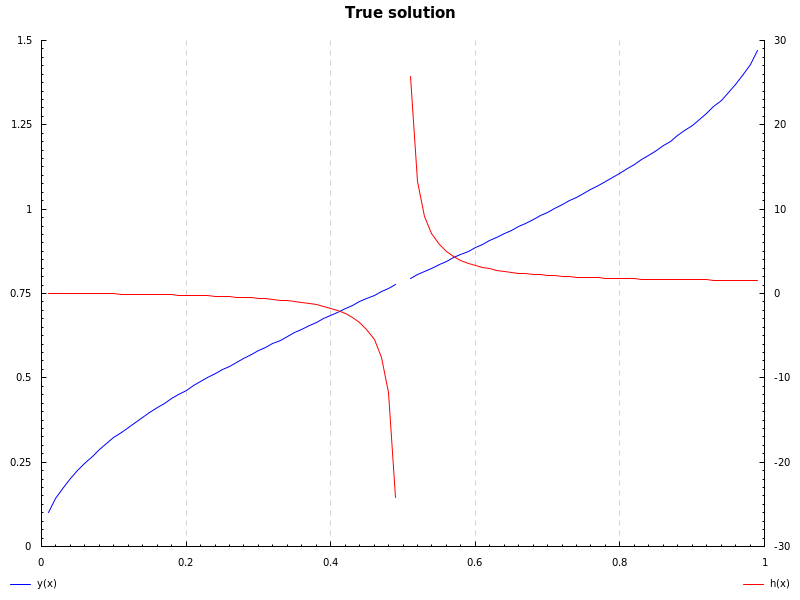
\includegraphics[scale=0.38]{solution}
\end{frame}

\begin{frame}{Сравнение методов : Метод Рунге-Кутта при делении отрезка на 1000 частей}
    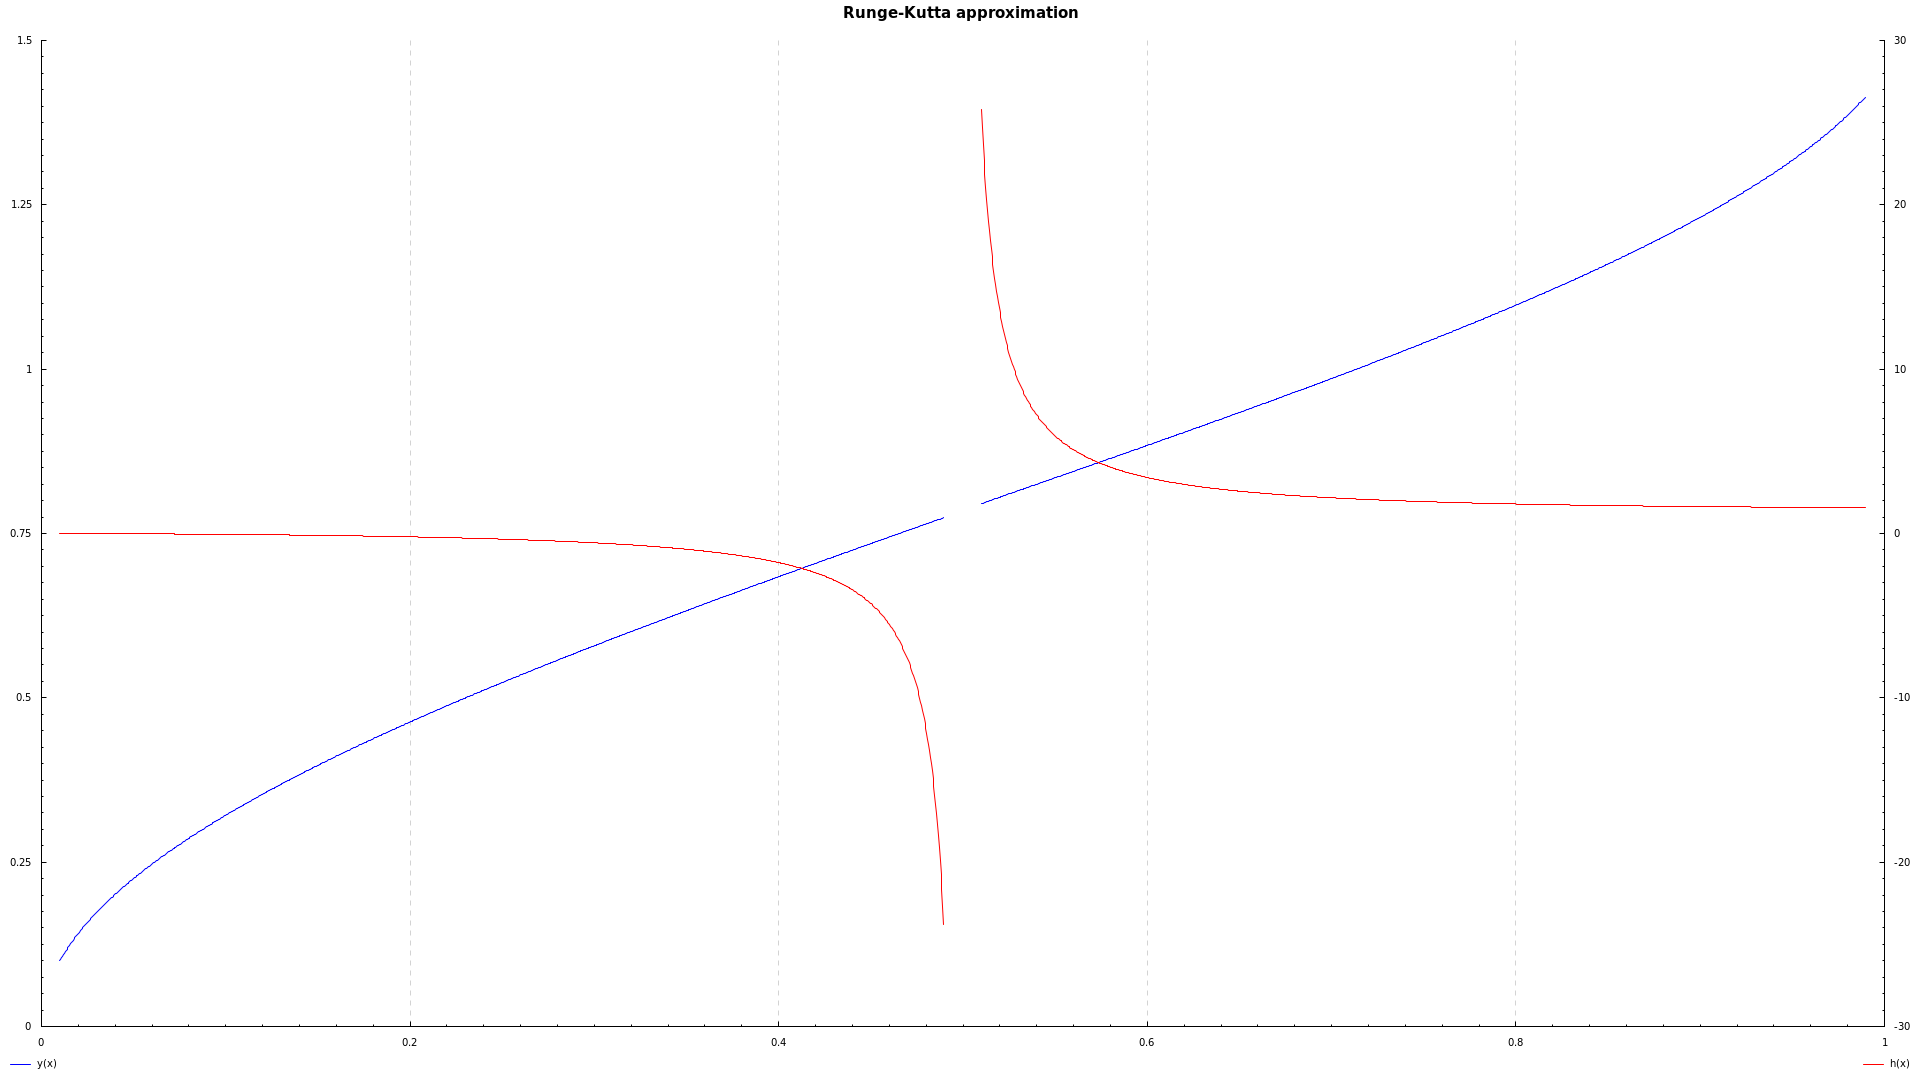
\includegraphics[scale=0.38]{runge1000}
\end{frame}


\begin{frame}{Сравнение методов : Метод Рунге-Кутта при делении отрезка на 50 частей}
	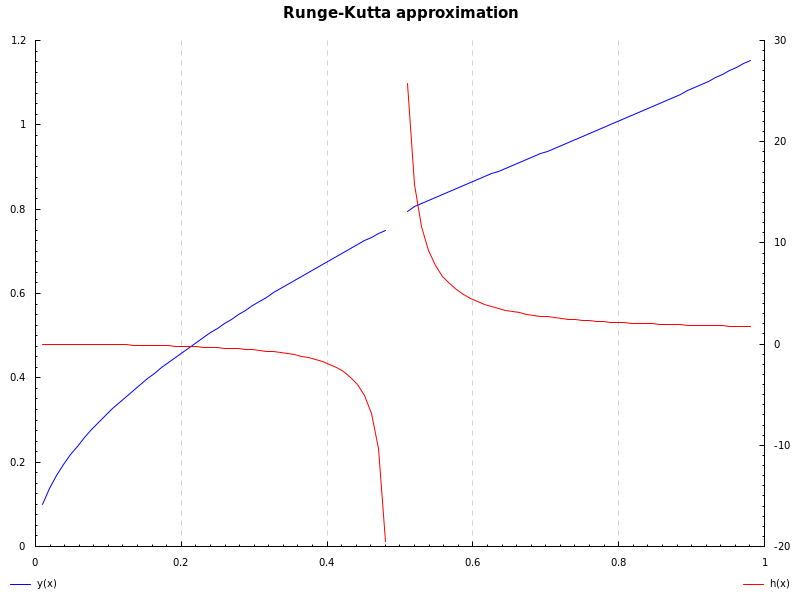
\includegraphics[scale=0.38]{runge50}
\end{frame}

\begin{frame}{Сравнение методов : Метод Эйлера при делении отрезка на 1000 частей}
    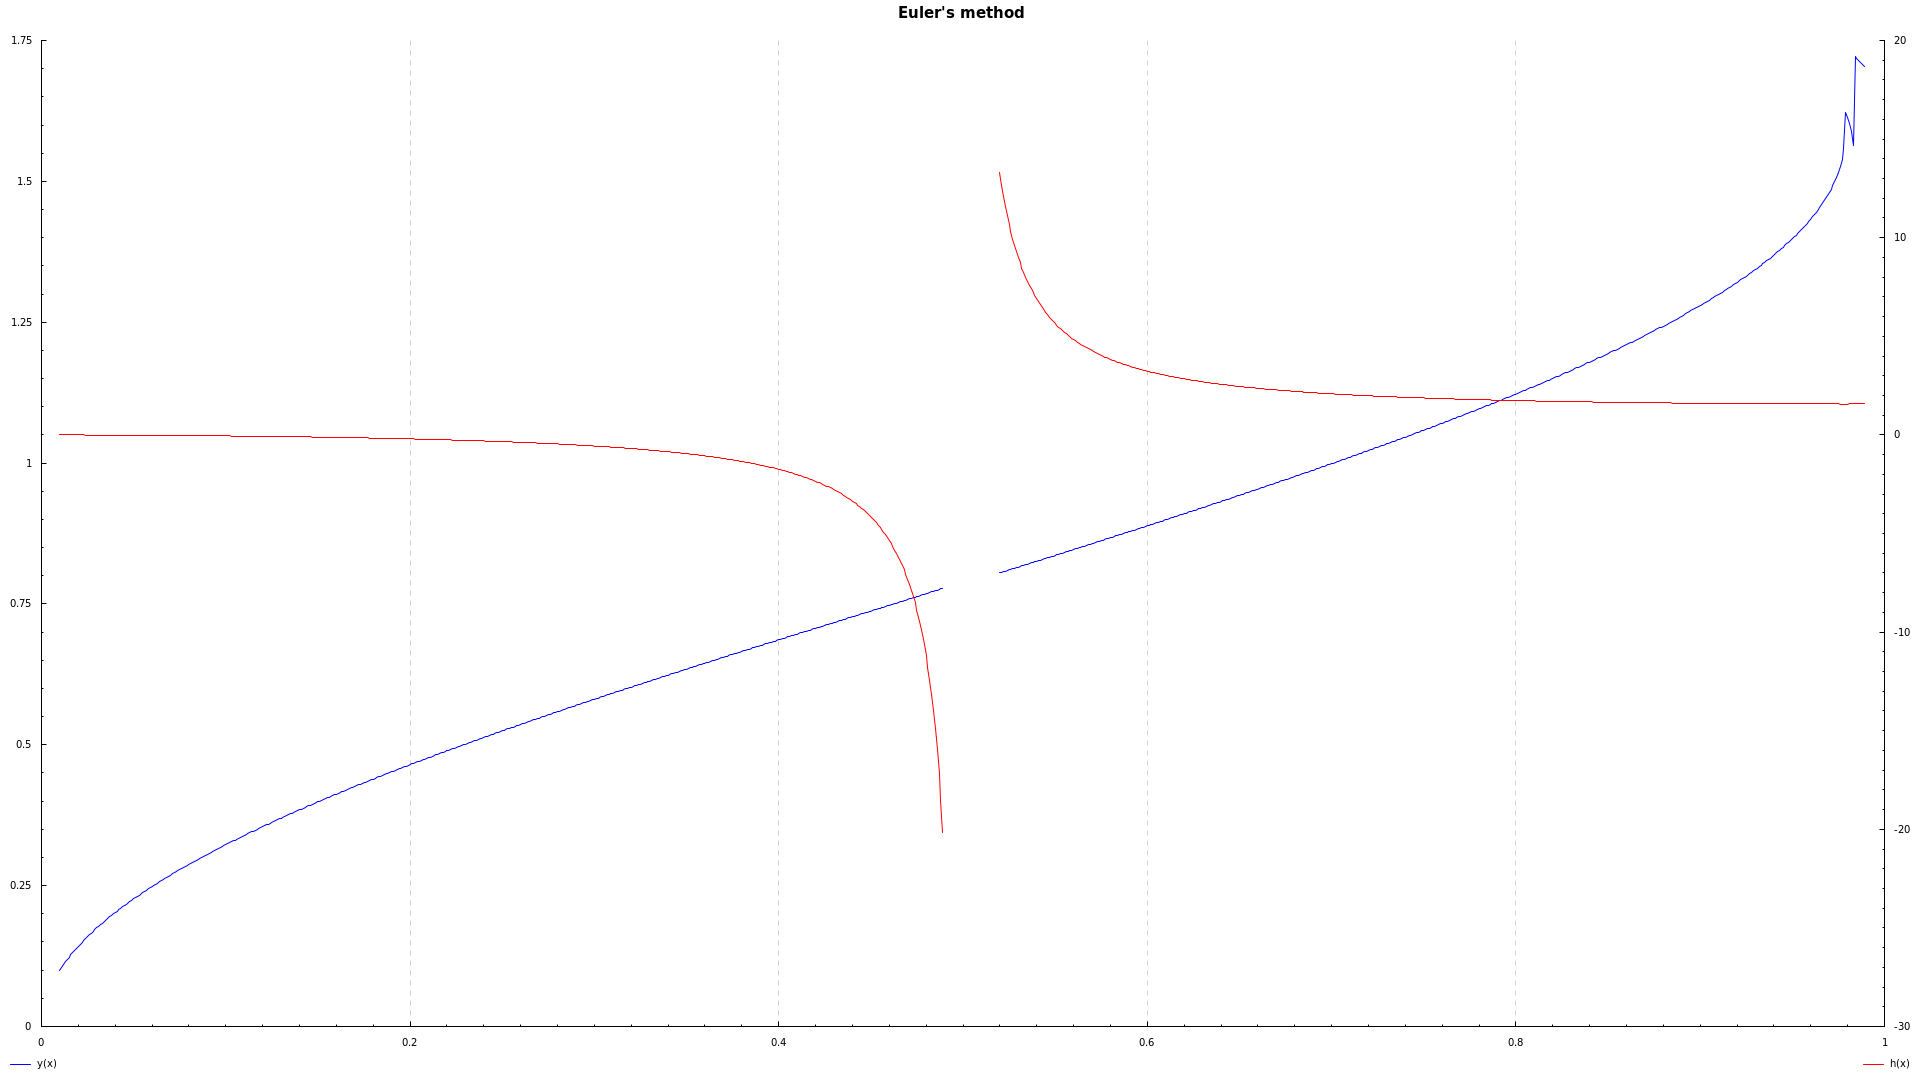
\includegraphics[scale=0.38]{euler}
\end{frame}

\begin{frame}{Анализ графиков}
    \begin{enumerate}
        \item Как мы можем видеть метод Рунге-Кутта дает решение почти неотличимое от настоящего при достаточно маленьком размере шага.
        \item Метод Эйлера, который является методом 2 порядка, дает хорошие графики только при достаточно маленьком шаге(можно сравнить вывод метода Рунге-Кутта при 50 точках и Эйлера при 1000). Это объясняется тем, что метод Рунге-Кутта имеет больший порядок точности.
    \end{enumerate}
\end{frame}




\end{document}
